\section{Narzędzia rysowania i edycji}
\label{sec:narzedzia_rysowania_i_edycji}

W celu umożliwienia użytkownikowi projektowania schematów układów scalonych,
w grze zaimplementowano zestaw narzędzi do rysowania i edycji, których założenia przedstawiono w podrozdziale~\ref{sec:zalozenia_funkcjonalne}.
Podobnie jak w przypadku warstw, narzędzia są wstępnie definiowane w pliku konfiguracyjnym SO, \texttt{ToolConfig}.
Zawiera on informacje o wskazówce dla narzędzia, ikonie, przypisanym klawiszu czy jest używane do edytowania zaznaczenia
oraz o grafice i hotspocie kursora niestandardowego kursora.
Przykładową konfigurację przedstawiono na rys.~\ref{fig:tool_config}.

\begin{figure}[h!]
    \centering
    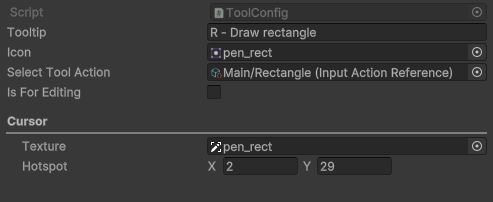
\includegraphics[width=0.9\textwidth]{chapters/chapter4/rys/tool_config}
    \caption[Przykładowa konfiguracja narzędzia.]{Przykładowa konfiguracja narzędzia, źródło: opracowanie własne.}
    \label{fig:tool_config}
\end{figure}

Narzędziami zarządza \texttt{ToolsManager}, odpowiadający za wybór aktywnego narzędzia,
a także zmianę ikony kursora w zależności od wybranego narzędzia.
Implementuje on także klasę \texttt{MonoSingleton}, aby ułatwić dostęp do niego z innych komponentów.
Ze względu na większą autonomię narzędzi w porównaniu do warstw,
dla każdego z nich stworzono osobny obiekt na scenie, z którym związane są wszystkie operacje rysowania lub edycji.
Wspólnym rodzicem narzędzi jest obiekt \texttt{Tools}, na którym znajduje się \texttt{ToolsManager},
rys.~\ref{fig:tools_hierarchy}.

\begin{figure}[h!]
    \centering
    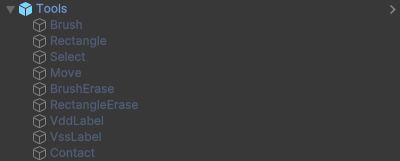
\includegraphics[width=0.9\textwidth]{chapters/chapter4/rys/tools_hierarchy}
    \caption[Hierarchia obiektów narzędzi na scenie.]{Hierarchia obiektów narzędzi na scenie, źródło: opracowanie własne.}
    \label{fig:tools_hierarchy}
\end{figure}

%\begin{figure}[h]
%    \centering
%    \begin{subfigure}{.45\textwidth}
%        \centering
%        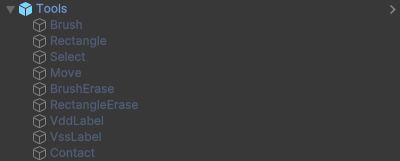
\includegraphics[width=.5\linewidth]{chapters/chapter4/rys/tools_hierarchy}
%        \caption{Hierarchia obiektów narzędzi na scenie.}
%        \label{fig:tools_hierarchy}
%    \end{subfigure}
%    \begin{subfigure}{.45\textwidth}
%        \centering
%        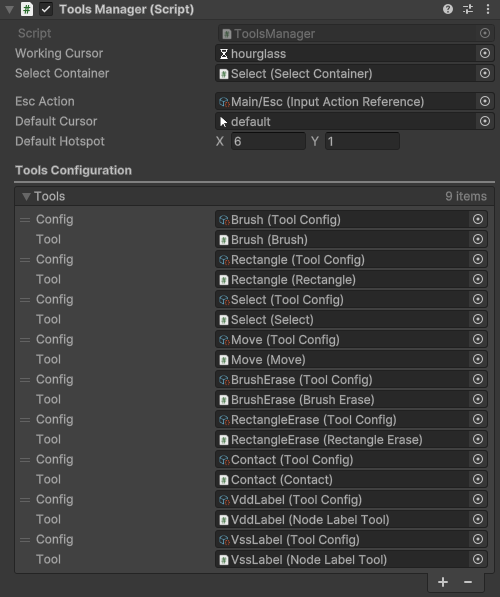
\includegraphics[width=.5\linewidth]{chapters/chapter4/rys/tools_manager}
%        \caption{Widok inspektora menedżera narzędzi.}
%        \label{fig:tools_manager}
%    \end{subfigure}
%    \caption[Widok narzędzi na scenie oraz inspektora komponenetu zarządzającego nimi.]
%    {
%        Widok narzędzi na scenie oraz inspektora komponenetu zarządzającego nimi,
%        źródło: opracowanie własne.
%    }
%    \label{fig:tools}
%\end{figure}

\newpage % TODO: check this if something changes

Ponieważ narzędzia są od początku obecne na scenie do \texttt{ToolsManager},
należało przypisać referencje konfiguracji narzędzi wraz z samymi narzędziami,
jak pokazano na rys.~\ref{fig:tools_manager}.
W tym celu stworzono dodatkowo strukturę \texttt{ToolHolder},
która przechowuje obie referencje.

\begin{figure}[h!]
    \centering
    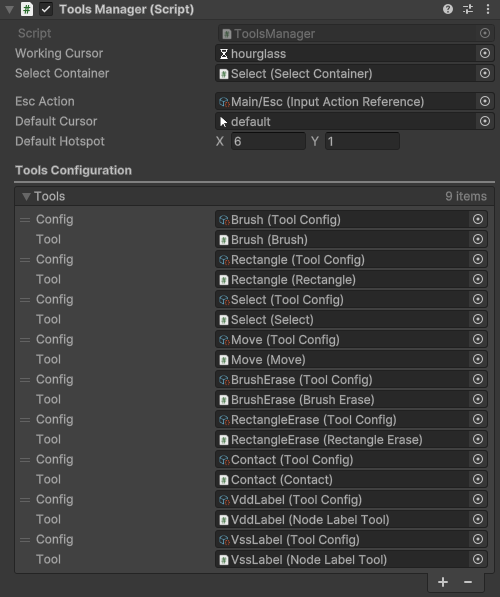
\includegraphics[width=0.9\textwidth]{chapters/chapter4/rys/tools_manager}
    \caption[Widok inspektora menedżera narzędzi.]{Widok inspektora menedżera narzędzi, źródło: opracowanie własne.}
    \label{fig:tools_manager}
\end{figure}

Wśród narzędzi można wyróżnić dwa główne typy różniące się pod kątem sposobu działania, punktowe i obszarowe.
Ze względu na ten podział korzystają one również z innych funkcji w celu wykrywania komórek.
Narzędzia punktowe działają jedynie na jedną komórkę jednocześnie,
z tego powodu do wykrywania komórek używają funkcji \texttt{Physics.Raycast}.
Sprawdza ona, czy w prostej linii występuje kolizja z obiektem posiadającym komponent \texttt{Collider}.
W przypadku narzędzi obszarowych wykrywanie odbywa się poprzez rozciąganie detektora w narzędziu,
którym jest \texttt{BoxCollider} z zaznaczoną opcją \textit{Is Trigger}.
W momencie kolizji z komórką wywoływana jest funkcja \texttt{OnTriggerEnter} w narzędziu,
która zwraca referencję do komórki, z którą nastąpiła kolizja.
Po wyjściu z kolizji wywoływana jest funkcja \texttt{OnTriggerExit}.
Dzięki wykorzystaniu tych funkcji możliwe jest wykrywanie komórek w trakcie pracy narzędzia,
przez co nie ma potrzeby znajdywania ich wszystkich w jednym kroku.
